\section{Initial investment}

\subsection{Description of the systems}

\paragraph{}A S-band system will be used for telemetry and telecommand purposes and for receiving housekeeping data. It is intended to have uplink and downlink capabilities in half-duplex.
\begin{figure}[H]
\begin{center}
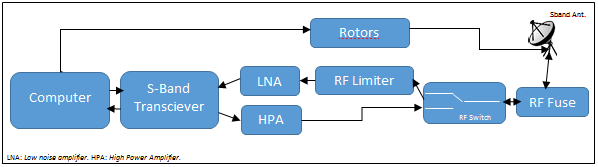
\includegraphics[scale=1]{SbandEquip.PNG}
\caption[S-band Equipment]{Equipment needed for S-band communications.}
\label{fig:SbandEquip}
\end{center}
\end{figure}

\paragraph{}A X-band system will be used for receiving the data requested by the client from the satellites. It will only have downlink capabilities.
begin{figure}[H]
\begin{figure}[H]
\begin{center}
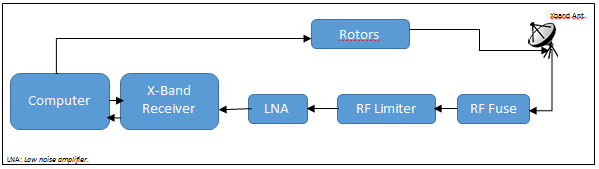
\includegraphics[scale=1]{XbandEquip.PNG}
\caption[X-band Equipment]{Equipment needed for X-band communications.}
\label{fig:XbandEquip}
\end{center}
\end{figure}

\subsection{Costs}

\paragraph{}The following items are needed:
\begin{itemize}
\item S-band system: 46,500\euro
\item X-band system: 100,000\euro
\item Computers and office material: 13,000\euro
\item Building: 50,000\euro
\end{itemize}

\paragraph{}Because of the time interval in which an antenna will be reorientating itself to point to the next satellite when the current satellite gets out of range, that antenna will not function until it finishes the reorientation. For this reason, two S-band and X-band systes are required for each ground station to be always operative. Therefore, each ground station needs two X-band systems, two S-band systems, computers and office material and a building.

\paragraph{}The initial investment of one ground station will be 356,000\euro . The initial investment of the three ground stations will be 1,070,000\euro .

\paragraph{}For the Mission Control Centre, the following costs are assumed:
\begin{itemize}
\item Computers and office material: 50,000\euro
\item Building: 100,000\euro
\end{itemize}
\paragraph{}The initial investment of the mission control centre will be 150,000\euro . The initial investment of all the ground segment will be 1,220,000\euro .